\documentclass[annual]{acmsiggraph}
\usepackage{wrapfig}
\title{XToon}

\author{Robert Wolfe\thanks{e-mail:robert\_wolfe@carleton.ca}\\Spencer Elliott\thanks{e-mail:spencer\_elliott@carleton.ca}}
\pdfauthor{Robert Wolfe, Spencer Elliott}

\keywords{xtoon, image processing, xna}

\begin{document}

\maketitle

\begin{abstract}

We are implementing XToon ~\cite{BTM06a}.

\end{abstract}

\keywordlist

\copyrightspace

\section{Introduction}

We first developed a standard cel shader using ~\cite{CelShadingTut}.

We used the GUI framework for XNA from ~\cite{Ruminate}.

\section{Tone Detail}
\begin{wrapfigure}{r}{0.1\textwidth}
  \vspace{-20pt}
  \begin{center}
    
\includegraphics[width=0.1\textwidth]{images/xtoon_skin}
  \end{center}
  \caption{2D Texture.}
  \vspace{-10pt}
  \label{fig:2dtexture}
\end{wrapfigure}
We extend the concept of a regular toon shader by adding a second dimension to the texture. While the x-axis remains as $n\cdot l$, as in a classic toon shader, the y-axis represents the level of detail. The higher up on the axis, the less detail is used. Conversely, the lower the y-axis value, the more detail. An example of a 2D texture used in this application can be seen in Figure~\ref{fig:2dtexture}.

The method of computing the y-axis depends on an {\it{attribute map.}} The chosen attribute changes the level of detail, depending on its value. The original paper provided two possible attribute maps: distance and orientation. We implement distance, and probvide a new attribute map based on angle.

\subsection{Distance}
{\bf*{* Spencer to write in here**}}

We use the distance along the focal axis to determine. Also light directions are used somehow.

\subsection{Angle}
We introduce a new attribute map based on the angles of the {\it{look at}} of the camera and the surface normal. The look at vector is the direction that the camera is pointed. The angle between the two vectors is calculated using Equation~\ref{eqn:angle}, which is derived from the formula for dot product.

\begin{equation}
\label{eqn:angle}
a = \cos^{-1}{(-LookAt \cdot Normal / |LookAt||Normal|)}
\end{equation}



\section{Results}
Here are some results

\begin{figure}[ht]
  \centering
  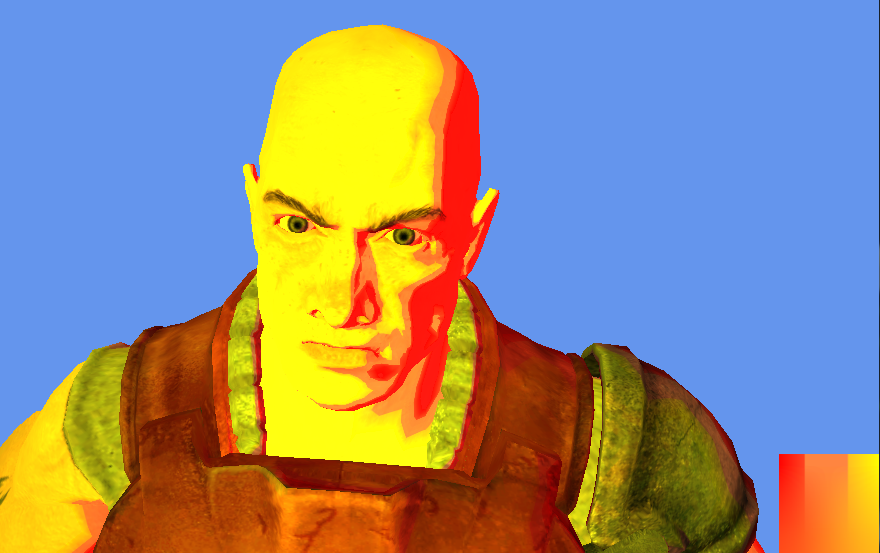
\includegraphics[width=2.5in]{images/test}
  \caption{Sample illustration.}
\end{figure}


\section{Discussion and Future Work}

Lorem ipsum dolor sit amet, consectetur adipisicing elit, sed do
eiusmod tempor incididunt ut labore et dolore magna aliqua. Ut enim ad
minim veniam, quis nostrud exercitation ullamco laboris nisi ut
aliquip ex ea commodo consequat. Duis aute irure dolor in
reprehenderit in voluptate velit esse cillum dolore eu fugiat nulla
pariatur. Excepteur sint occaecat cupidatat non proident, sunt in
culpa qui officia deserunt mollit anim id est laborum.

Lorem ipsum dolor sit amet, consectetur adipisicing elit, sed do
eiusmod tempor incididunt ut labore et dolore magna aliqua. Ut enim ad
minim veniam, quis nostrud exercitation ullamco laboris nisi ut
aliquip ex ea commodo consequat. Duis aute irure dolor in
reprehenderit in voluptate velit esse cillum dolore eu fugiat nulla
pariatur. Excepteur sint occaecat cupidatat non proident, sunt in
culpa qui officia deserunt mollit anim id est laborum.

Lorem ipsum dolor sit amet, consectetur adipisicing elit, sed do
eiusmod tempor incididunt ut labore et dolore magna aliqua. Ut enim ad
minim veniam, quis nostrud exercitation ullamco laboris nisi ut
aliquip ex ea commodo consequat. Duis aute irure dolor in
reprehenderit in voluptate velit esse cillum dolore eu fugiat nulla
pariatur. Excepteur sint occaecat cupidatat non proident, sunt in
culpa qui officia deserunt mollit anim id est laborum.

Lorem ipsum dolor sit amet, consectetur adipisicing elit, sed do
eiusmod tempor incididunt ut labore et dolore magna aliqua. Ut enim ad
minim veniam, quis nostrud exercitation ullamco laboris nisi ut
aliquip ex ea commodo consequat. Duis aute irure dolor in
reprehenderit in voluptate velit esse cillum dolore eu fugiat nulla
pariatur. Excepteur sint occaecat cupidatat non proident, sunt in
culpa qui officia deserunt mollit anim id est laborum.

Lorem ipsum dolor sit amet, consectetur adipisicing elit, sed do
eiusmod tempor incididunt ut labore et dolore magna aliqua. Ut enim ad
minim veniam, quis nostrud exercitation ullamco laboris nisi ut
aliquip ex ea commodo consequat. Duis aute irure dolor in
reprehenderit in voluptate velit esse cillum dolore eu fugiat nulla
pariatur. Excepteur sint occaecat cupidatat non proident, sunt in
culpa qui officia deserunt mollit anim id est laborum.

\section{Conclusion}

Lorem ipsum dolor sit amet, consectetur adipisicing elit, sed do
eiusmod tempor incididunt ut labore et dolore magna aliqua. Ut enim ad
minim veniam, quis nostrud exercitation ullamco laboris nisi ut
aliquip ex ea commodo consequat. Duis aute irure dolor in
reprehenderit in voluptate velit esse cillum dolore eu fugiat nulla
pariatur. Excepteur sint occaecat cupidatat non proident, sunt in
culpa qui officia deserunt mollit anim id est laborum.

\bibliographystyle{acmsiggraph}
\bibliography{paper}
\end{document}
